\documentclass{tufte-handout}

\title{Utility Theory and the Representation of Preference}

\author[Nathaniel Forde]{Nathaniel Forde}

%\date{28 March 2010} % without \date command, current date is supplied

%\geometry{showframe} % display margins for debugging page layout

\usepackage{graphicx} % allow embedded images
  \setkeys{Gin}{width=\linewidth,totalheight=\textheight,keepaspectratio}
  \graphicspath{{graphics/}} % set of paths to search for images
\usepackage{amsmath}  % extended mathematics
\usepackage{booktabs} % book-quality tables
\usepackage{units}    % non-stacked fractions and better unit spacing
\usepackage{multicol} % multiple column layout facilities
\usepackage{lipsum}   % filler text
\usepackage{fancyvrb} % extended verbatim environments
  \fvset{fontsize=\normalsize}% default font size for fancy-verbatim environments
\usepackage{minted}
\usepackage{mathtools}
\usepackage[math]{cellspace}
\usepackage[most]{tcolorbox}
\usepackage{tikz}
\usepackage{stmaryrd}
\usepackage{mdframed}
\newtheorem{theo}[section]{Theorem}
\usepackage{hyperref}
\hypersetup{
    colorlinks=true,
    linkcolor=blue,
    filecolor=magenta,      
    urlcolor=cyan,
}

\newenvironment{ftheo}[1]
  {\begin{mdframed}
  \sloppy
  \begin{theo}[#1]
  }
  {\end{theo}
\end{mdframed}}

% Standardize command font styles and environments
\newcommand{\doccmd}[1]{\texttt{\textbackslash#1}}% command name -- adds backslash automatically
\newcommand{\docopt}[1]{\ensuremath{\langle}\textrm{\textit{#1}}\ensuremath{\rangle}}% optional command argument
\newcommand{\docarg}[1]{\textrm{\textit{#1}}}% (required) command argument
\newcommand{\docenv}[1]{\textsf{#1}}% environment name
\newcommand{\docpkg}[1]{\texttt{#1}}% package name
\newcommand{\doccls}[1]{\texttt{#1}}% document class name
\newcommand{\docclsopt}[1]{\texttt{#1}}% document class option name
\newenvironment{docspec}{\begin{quote}\noindent}{\end{quote}}% command specification environment
\definecolor{myblue}{RGB}{3,81,138}
\definecolor{mygray}{RGB}{236, 236, 236}

\tcbset{mystyle/.style={
  breakable,
  enhanced,
  outer arc=0pt,
  arc=0pt,
  colframe=myblue,
  colback=mygray,
  attach boxed title to top left,
  boxed title style={
    colback=myblue,
    outer arc=0pt,
    arc=0pt,
    },
  fonttitle=\sffamily
  }
}

\newtcolorbox[auto counter,number within=chapter]{example}[1][]{
  mystyle,
  title= Box~\thetcbcounter:#1
}

\renewcommand{\contentsname}{Utility Representation - Table of Contents}

\begin{document}

\tableofcontents

\maketitle% this prints the handout title, author, and date


\noindent The average man is a melange of imagined parts. A Frankenstein's monster of mismatched limbs, variously soldered, stapled or sown at the joints. Such were the fears of the mathematician Augustin Cournot in the 1840s. He worried that no one but a "physical monstrosity" could exhibit the average, weight, height and other attributes in one body. But fantastical fears were no bar to a useful mathematical fiction. The applications of averaging multiplied without cease: polling, gambling, forecasting - statistics were recorded everywhere, compounding one on another; averages of averages tenuously tethered to observable facts by layers of abstraction and scales of measurement. Slowly, some doubts began to surface again. \cite{stigler2016seven} Many decades later in the 1970s the psychologist Paul Meehl would worry that such brute approximations had stifled the development of the softer sciences and contributed to the mis-measurement of man. He would go on to elaborate twenty features of psychological science which made such measurement constructs inapt, unreliable and difficult to clearly falsify. This was progress! \cite{MeehlTheoretical} He then showed that the methods of validating such constructs were the main culprit and the likely cause of psychology's implausible claims to concrete, replicable results. Around thirty years later some of the same replication issues would come to be called a crisis.
\linebreak

\noindent Seen from the perspective of a patient the difficulties are even more stark.

\section{\textbf{Expected Value: Explanation and Target}}
\label{sec:Expectations}

There is an algorithm beloved by bureaucrats. An unsung hero of administrators and accountants. An algorithm both ubiquitous and under appreciated. It's pivotal for nearly every project and informs the actions of tech firms and policy makers the world over. It is only mildly hyperbolic to say that understanding this formula unlocks wealth and power. The algorithm lies at the heart of online A/B testing, all policy analysis, sound business strategy and poker play. 
$$ EV(O)_{p} = p_{1}u(o_{1}) + p_{2}u(o_{2}) + ... + p_{k}u(o_{k}) $$
The expected financial value of a random process is just the sum of the utility (typically dollar outcomes) weighted by their probabilities. 
Outcomes can vary from deals of cards, to customer transactions and election results. Aside from the mercenary possibilities, Pascal can argue sincerely that such considerations compel belief in God. The infinite downsides of hell at any likelihood ought to compel even the cynical sceptic.  But the formula, glossed as a rule for rational action, merits your attention for more mundane wagers too. If you intend to maximise your expected value, the meaning of probability is not an idle concern.\footnote{For a typical example of how $EV$ is used to express decisions under uncertainty see chapter 7 in the textbook \cite{BarberBR_ML}} While statistics are often tortured to rubber stamp decisions and probabilities are abused to fit policy prescriptions with false precision, the crisp clarity of the rule has an enduring appeal that promises to sift the murky swamps of Big Data. It's a scalpel that anyone can wield to parse the syntax of statistical jargon and carve answers from an abstract space of probabilities. "What's my expected return?" - a simple question, with a surprisingly complex answer. 
\linebreak

\noindent Whenever expected value is used as a KPI there is a pivot point in the journey where an explanatory model of rational expected action is substituted for more obscure black-box techniques. The focus switches from modelling the consumer to modelling returns based on the consumer and the firms expected value. Swapping a customer catering model for a customer-as-commodity perspective focused on profit and customer acquisition. The tendency is common because profit is tempting and often overwhelms all other priorities, but the loss of understanding typically amounts to a longer term net-loss. Increased relative profit and algorithms deployed at scale can give comfort to shareholders, but it's rare that any single algorithm actually or always maximises the available profit. This dynamic enforces a kind of inescapable see-saw motion where the consumer modelling exercise goes through a constant feedback loop. A good model (informal or formal) of customer needs and wants feeds a better a predictive model of customer action. When the latter fails we go back to the utility curves and the algorithm of expected value because it is (if not reliably predictive) a rich and deeply explanatory model of human action under uncertainty. 

\section{\textbf{Part I: Probability Measures}}

\subsection{Probability: Two sides of a Coin}
\label{sec:Probability}
Probability emerged slowly and with a dual aspect. On one tradition it refers to the long run tendency of a random process, on another probability is construed as the degree of belief in an outcome. On the first (frequentist) interpretation a probability distribution has certain fixed theoretical characteristics: as in a uniform probability distribution of a fair coin where all outcomes are equally likely, or as with the normal distribution where most outcomes cluster symmetrically about a central average. On the second (Bayesian) reading the characteristics of the probability distribution are learned from the data. The controversy centres around the fact that it's unclear how a frequentist could ascribe probabilities to unique events. Without appeal to a large set of observations (or known theoretical distribution) the claim that an event appears frequently or infrequently is not well defined. Consequently, tabulations of probability appear inappropriate for claims of unique or rare events. In contrast the Bayesian is content to ascribe probabilities to any all partial beliefs no matter how specific. For the Bayesian, the probability calculus is a set of edicts about how to rationally manage and modulate your beliefs. So it's acceptable to have a probabilistic belief in rare cases so long as you update those probabilities with new data when available. \linebreak 

\noindent These two approaches are united by the Law of Large numbers which states that as the size of our sample increases our sample average will converge to the expected realisation of the theoretical process. 
$$  \frac{1}{N} \sum_{i = 1}^{N} O_{i} \text{ converges to }  E(O) \text{ as } N \text{ approaches } \infty $$ 
\begin{marginfigure}
  \includegraphics[width=\linewidth]{../Expectation/Plots/convergence_of_law_of_large_numbers.png}
  \caption{Convergence with large samples}
\end{marginfigure}

\noindent In this graph (Figure 1) we have fixed a Poisson distribution with a mean of 4.5 and can see three examples of how consecutive averaging from the increasing sample sizes results in a closer and closer convergence to the (true) population mean. Though common knowledge today, in 1650 ``the very concept of averaging is [new]... and most people could not observe an average because they did not take averages.''\cite{HackingEmergence} Grappling with the implications of observations is a somewhat recent human endeavour - one which is far from perfected. This tendency is now fundamental to the interpretation of probability. Take a game with fixed and fair odds and we see that repeated play will converge over time because of characteristics which govern the process. Dice are a homely example. In the wild we never know the characteristics which cause the observed spread of outcomes, but such is the influence of gambling on probability, that we assume there exists a stable pattern to be gamed. Partially this is pragmatic, the maths is more tractable if we can assume a well behaved underlying process. The results are compelling: The Normal (Bell Curve) distribution, the Poisson distribution the Bernoulli distribution (to name a few) are all rightly famous. Their shapes are characteristics of innumerable random processes. They cleanly circumscribe and corral the likely patterns of events. 
\linebreak
\begin{marginfigure}
  \includegraphics[width=\linewidth]{../Expectation/Plots/variety_of_distributions.png}
  \caption{Some theoretical distributions with parameters}
\end{marginfigure}

\noindent But the gambling paradigm clouds the fact that in practice we start on the left side of the law of large numbers (with samples) and we often start with small numbers resulting from a unknown number of data-generating processes. Well behaved probability distributions are rare beasts; a tiny fraction of the world's arbitrary menagerie. The fundamental question in probability is not whether probability is a measure of belief or frequency - it is whether we can safely assume that the underlying process adheres to a known model? The Bayesian focus is to try and learn from the new data the expected characteristics of the underlying process, while the Frequentist tries to gauge the accuracy of their assumptions about the underlying process. Both are attempts to validate the structure of the model's theoretical distribution to inform inference. If we can't validate a model, we're better learning what we can from the sample, trusting to wide confidence intervals and worst scenario planning. But in all cases the following questions are inescapable when we need to make a decision: What are your expectations based on? How do they figure in our choices, and can we use them to improve our outcomes? 

\subsection{Small Worlds and Statistical Inference}
\label{sec:Inference}
Prediction is a visceral need, it precedes probability in any order of analysis. Without some regularity between $X, Y$ we can only interpret their collisions as timorous noise. Only when there is a better than arbitrary correlation between $X, Y$ will we think to ascribe a measurable probability to their association. So whether we view probabilities as a measure of credibility or frequency, the focus is always on a process which in reality reveals a pattern under repetition. We're loath to apply a probability model of any kind without some base inductive evidence. Models then are deliberate simplifications of complexity. Attempts to formulate a unobserved process within a mathematical structure. Lego-like versions of the world are built and rebuilt, in which we bash parts together to see what reliably sticks. Forget about the pieces we don't own. Count the pairs of blocks that: match, wedge, smash, click-into-place or break, then draw out the ratio of success and the spread of outcomes. Parse out the details of how reds go with greens, and blues with yellows. This is your sample distribution. The expected revenue depends on both this uncertainty measured in this small world and the finer points of statistical inference.\footnote{A [small world] is... completely satisfactory, only if it is actually a microcosm, that is, only if it leads to a probability measure ... that can be written down explicitly pg 88 \cite{savage54}}
\linebreak

\noindent Statistical models are mostly machines for figuring out expected values of a statistical process. There can be multiple plausible approximations of the underlying process which need to be assessed comparatively on their ``goodness" of fit. We iterate through new and improved versions, each an attempt to make a conjectural connection between $ X, Y $ mathematically precise. Consider how a basic regression model tries to predict an outcome $Y$ as linear function of some observed features $X$:

$$ Y = const + \beta X + \epsilon  \ $$

\noindent where $\epsilon$ is a random variable representing the error (or noise). A modest notational device for disaster. While $const, \beta$ are parameters estimated by an optimisation process to ensure the equation fits the data as neatly as possible. In (Figure 3) below we have a series characterised by change. After the first shock we can refit the model so that the line tracks well with the evolving data. After the second shock we try another refit, but the range the and variance of the data makes our basic model a poor fit, i.e. the data no longer exhibits a linear relationship. This presents three examples of error in the modelling process: (i) it's difficult to identify (in the moment) those changepoints in the data which reflect structural change, (ii)  the linearity assumptions that go into the model are sound but the parameters need be re-estimated based on the new data and (iii) the third linear model is simply a terrible match for the pattern in the data.
\linebreak 
\begin{marginfigure}
  \includegraphics[width=\linewidth]{../Expectation/Plots/piecewise_linear_fits.png}
  \caption{Three samples with starkly different parametrisations}
\end{marginfigure}


\noindent Every model is a guess as to the implicit order in apparent noise. Sometimes there is no order, and other times the patterns is too subtle for a dumb model to capture. In practice you never really know whether a single new error stems from a misfit but appropriate model or an entirely inappropriate model. As we increase our number of sample fits we hope to better approximate the true linear process (if any) generating the data. Imagine now that the data points in Figure 3 are repeatedly re-speckled over the canvas. We can refit a new model for each set of scattered data points and each refit gives us a new sample values for $ const, \beta$. If the underlying data generating process is stable, then the parameter fits will converge to the correct values of $const, \beta$; correct in the sense that they can be used to draw the line of best fit for the data. A statistically stable process is one that can be modelled with errors $\epsilon$ normally distributed around $0$, so that the model will be \textit{ correct on average} because $E(\epsilon) = 0$. Our predictions will overshoot in some cases but on the whole the errors up and down will cancel each other out. Forecasting with the parameters of best fit minimises our forecast errors because the fluctuations are stable about the centre of the line. These are the required assumptions for a process to exhibit the tendency of regression towards the mean. If they're not met, we will see poor parameter estimates and wild swings away from the linear path.\footnote{``Typically, the assumptions in a statistical model are quite hard to prove or disprove, and little effort is spent in that direction. The strength of empircal claims made on the basis of such modeling therefore does not derive from the solidity of those assumptions. Equally, these beliefs cannot be justified by the complexity of the calculations... These observations lead to uncomfortable questions"\cite{freedman_2009}}

\subsection{Modeling: Improper Assumptions and Skewed Expectations}

\noindent Below we build two sampling distributions based on different models of an underlying processes.  One in which the errors are independent, normally distributed around $0$ and in the other the errors are correlated in a sine-wave like pattern, increasing and decreasing periodically. This is akin to the difference between measuring error when predicting the heights of randomly sampled people versus predicting the sales volumes on randomly selected days of the week. A random sample of daily sales risks clumping weekends together and skewing the expected values. No such risk exists when sampling from independent individuals. 

\begin{minted}{python}
### Build True Models
N = 100000
X = random.uniform(0, 20, N)
independent_err = random.normal(0, 10, N)
corr_err = random.uniform (0, 10) +  sin(np.linspace(0, 10*pi, N)) +
sin(np.linspace(0, 5*pi, N))**2 +  sin(np.linspace(1, 6*pi, N))**2

Y_corr = -2 + 3.5 * X + corr_err
Y = -2 + 3.5 * X + independent_err

population = pd.DataFrame({'X': X,  'Y': Y, 'Y_corr': Y_corr})

### Sample from Data 
### and build smaller models

fits = DataFrame(columns=['iid_const', 'iid_beta', 'corr_const', 
 'corr_beta'])
 
for i in range(0, 10000):
    sample = population.sample(n=100, 
    replace=True)
    Y = sample['Y']; X = sample['X']
    Y_corr = sample['Y_corr']
    X = add_constant(X)
    iid_model = OLS(Y, X)
    results = iid_model.fit()
    corr_model = OLS(Y_corr, X)
    results_2 = corr_model.fit()
    row = [results.params[0],  results.params[1], 
           results_2.params[0], results_2.params[1]]
    fits.loc[len(fits)] = row
    
fits.boxplot()
\end{minted}

\begin{marginfigure}
  \includegraphics[width=\linewidth]{../Expectation/Plots/distribution_of_beta1.png}
  \caption{The expected realisations for $\beta, const$ with different errors structures}
\end{marginfigure}

\noindent In the case with independent errors the expected value for our parameter estimates match almost exactly the true values of the process. In the second model with correlated errors the parameter estimate for our constant is 4.9 which is significantly different from the true value of -2, and will lead to systematically skewed predictions. Statistical models are just algebraic equations where we use regular sampling to solve for $Y$ from $X$. Because Y is also a random variable the regression model encodes a conditional expectation result.

\begin{figure}
\begin{multicols}{2}
      \includegraphics[width=\linewidth]{../Expectation/Plots/errors_dist_iid.png}\par 
    \includegraphics[width=\linewidth]{../Expectation/Plots/correlated_errors_dist.png}\par 
    \end{multicols}
  \caption{Error Distribution for the two models on a random sample of 1000 observations}
\end{figure}

$$ E(Y_{i} | X_{i} = x )$$
For fixed values of X, the predictions $Y_{i}$ can be spread in a pattern enforced by the various ways we can realise the linear function with estimates for $\beta$ and $const$. But the regression model selects the best parameter values to minimise the squared prediction error and represent the conditional expected distribution of $Y$.\footnote{``The statement that regression approximates the [Conditional Expectation Function] lines up with our view of empirical work as an effort to describe the essential features of statistical relationships without necessarily trying to pin them down exactly" p38 - \cite{angrist_mostly_2008}} The consequent point predictions for $Y$ are always expected values, skewed by the how the parameters are realised from sample data as much as by poor choices in model design and predictive features. So too then any measures of expected revenue based on these models, and inferences from these distributions. 


\subsection{Frequentism: Inference from Expected Frequency}
Making inference from a model is delicate thing. Even simple cases come with controversy. Count the number heads in a series of 5 successive coin flips, then repeat the process 1000 times and you'll arrive at a proportion which characterises that process. If it's a fair coin the long run expected result will be half the number of your coin flips. If the coin is weighted you might have as few as 0. This is the binomial distribution, and it really shines when you're trying to gauge fairness. If a process is biased, the distribution will be skewed. We can use this fact for inference. Consider a dispute over whether the game was rigged. 
$$ H_0 : \text{ true proportion of heads } = 0.4  $$
$$ H_1 : \text{ true proportion of heads } =  0.5 $$

\begin{marginfigure}
  \includegraphics[width=\linewidth]{../Expectation/Plots/binomial_test.png}
  \caption{The Binomial Distribution}
\end{marginfigure}


\noindent Take $(H0)$ as given then if we observe a sequence: $$ (3in5): H, H, H, T, T$$ what does it say about the possibility that we're being hustled? If the coin is biased, then the count of heads in repeated sampling will reflect a clear bias. For any new data we can check if the data is consistent with the data generated by the biased coin. The pattern of reasoning is straightforward (i) make some assumptions about the structure of the random process under investigation, (ii) tease out the consequences of these assumptions (iii) evaluate the incoming data against these consequences to see if you need to revise your assumptions. The frequentist asks, does the data looks weird given the assumed shape of our probability distribution?\footnote{`` [I]n statistical terms $H_{0}$ [the null hypothesis] refers to a probability model and the very word `model' implies idealization. With a very few possible exceptions it would be absurd to think  that a mathematical model is an exact representation of a real system... We use the term to mean that in the current state of knowledge it is reasonable to proceed as if the hypothesis was true." pg 31 \cite{cox2006pos}}
\linebreak

\noindent In this instance the shape of the binomial distribution defined by a 0.4 biased coin allows for significantly greater than  5\% chance for observing the above sequence. So we do not have enough reason to reject $(H0)$ at the traditional threshold. By design the assumed distribution builds in characteristics of long-run variance of the process, and the slim threshold for rejection is designed to minimise incorrect rejections of $(H0)$. We should remain suspicious that we're being conned. However, with a low number of observations the sample distribution is unlikely to be properly representative. This makes even small p-value thresholds unreliable. We cannot blindly take a sample poll to imply the spread or volatility of a population, and with low or un-representative samples it's hard to justify any kind of inference from expectation, since we are not in a position to justify the choice of the null hypothesis either!

\subsection{Bayesian Inference: Inference to Expected Value}
If instead we use probability to calibrate our beliefs, then we can be more explicit in our assessment of $(H0), (H1)$. Let's assume that our prior beliefs about whether the game is rigged is 50/50. Then we evaluate the two hypothesis using Bayes's rule for incorporating our prior belief and the data. The Bayesian asks whether our hypothesis is a good explanation of the data compared to alternatives. How, upon observing the data, should we view our hypothesis?

$$ \overset{posterior}{p(H_{i} | Data)} = \frac{\overset{prior}{p(H_{i})}\overset{liklihood}{p(Data | H_{i})}}{\underset{evidence}{\sum_{i=1}^{i =K} p(Data | H_{i})p(H_i)}}$$

where $ 1 \leq i \leq K$ spans the ways in which the data could have been realised across all competing hypotheses. Then, in our toy example, we have:

$$ \frac{p(H_1 | 3 in 5)}{p(H_{0} | 3 in 5)} = \frac{\frac{.5\cdot .23}{.5\cdot .32 + .5 \cdot .23}}{\frac{.5\cdot .32}{.5\cdot .32 + .5 \cdot .23}} = \frac{.57}{.42} $$

\noindent which would lead us to infer that the coin was fair. The really radical move in the Bayesian setting is that you're allowed to ascribe a probability to any event regardless of whether there is any long-run sequence to observe. You may know nothing about your opponent or the coin, but for Bayesians this is no bar to assigning suspicion in the form of expected probability, so long as you act in accordance with the axioms of probability. It's this freedom which can seem arbitrary and unmotivated or even paradoxical, but in practice probabilities  are rarely ascribed entirely without reason. 


\subsection{An Example: Expected Website Returns}
Neither the Bayesian or Frequentist analysis ends with these simple calculations, both would continue to probe the limits of each hypothesis. We'd have to consider things like sample size and sensitivity testing, model performance and cost of errors, appropriateness of the priors. The point is just that there are reasons for dispute. Bayesian inference acts like a logic engine for evidence, whereas the frequentist approach is more focused on diagnosing the possibility of error. In general they are complementary methods, and when they conflict the assumptions should be scrutinised.  This example shows the heart of the conflict in the dual aspect of probability. There is enough latitude in the manner in which we set up a probability model that the mathematics of inference can yield inconsistent results.\linebreak

\noindent  The frequentist evaluation of our biased coin is very sensitive to the choice of hypotheses, while the Bayesian approach is influenced by the choice of prior. Why set up a significance test against assumed cheating rather than assumed fairness? Why attribute equal weight to both hypotheses? Why use a 5\% threshold if you're concerned about systematic cheating? Both offer strategies for managing uncertainty, but both approaches come with baggage. Consider a more concrete example.
\linebreak

\noindent Websites and apps collect traffic and log interactions. Your details are captured and pulled into vast aggregates of consumer data. I can route and re-route your trajectory across an online environment. Applying the same pressures to tens of thousands of others, we can trace out how the topology of particular sites throw up speed bumps on the customer's journey. Imagine we're running a website which aims to funnel customers through to a number of different purchase plans. The historic patterns are relatively stable with only 10\% of customers dropping out of our conversion funnel on a daily basis. We can sample actions online (Figure 7) under differing pressures with a view to evaluating expected values of repeated coercive prompts.
\linebreak

\begin{marginfigure}
  \includegraphics[width=\linewidth]{../Expectation/Plots/outcomes_of_signup.png}
  \caption{Stable long run Sign Ups }
\end{marginfigure}

\noindent Assume the particular values for each plan, then the expected value of customer journey is just: $ p_{1}\$(o_{1}) + p_{2}\$(o_{2}) + p_{3}\$(o_{3}) + p_{4}\$(o_{4})  = .3*\$10 + .4*\$7  + .2*\$12 + .1*\$0 = \$8.20.$ Now imagine there was a change to the website and we observe the following pattern (Figure 8) for the next 20 days:
\linebreak

\begin{marginfigure}
  \includegraphics[width=\linewidth]{../Expectation/Plots/outcomes_of_signup_post.png}
  \caption{Abrupt increase in dropouts}
\end{marginfigure}

\noindent What is the new expected value? From the frequentist point of view the macro distributional properties haven't significantly changed. But given what we know about the change to the website it would be foolish to assume such a static distributional assumption. Looking only at the small sample of new data, the variance will be large and the estimates of rates of sign-up for each plan will be unstable.  Following the Bayesian paradigm we can condition our expectations on the new data, the old data or all the data. The below graph illustrates the spread in values expected revenue calculated on different slices of our data using Bayes Rule.
\linebreak

\noindent Using a large number of observations, the influence of our priors are minimal and washed out by the data, giving us a strong point estimate with low variance stable around 8.2, but since the recent data involves a step change, we might be better off ignoring the old data. But we can also see that if we condition our expectations only on the new data with different priors drawn from the past data or hope, we can positively bias our expectations.
\linebreak

\begin{marginfigure}
  \includegraphics[width=\linewidth]{../Expectation/Plots/expected_revenue_distributions.png}
  \caption{Expected revenue differs by choice of prior and data}
\end{marginfigure}

\noindent Nearly all substantial decisions are made with small samples in circumstances where past behaviour is not a guide. Past behavioural patterns are exactly what we're trying to avoid or change. If you want to know whether the change on your website will drive a material change in financial revenue, you won't have long run patterns to rely on, and it's an open question on how to weight the new data. All models smuggle-in a host of statistical assumptions and these can be range from reasonable to absurd. Even when reasonable they're only supported by large sample sizes, and most questions of interest are driven by novelty (or specificity) that short circuits appeal to robust patterns of history. Reasoning from small samples is common, best done with caution and plenty of caveats, but better reason than not. Expectations should be modified accordingly.

\begin{marginfigure}
\includegraphics[width=3in]{Plots/utility_in_1_dimension.png}
\caption{Consumer attitudes with differently satisfied appetites for a good}
\includegraphics[width=3in]{Plots/derivatives_of_utility.png}
\caption{The Rates of Change of personal Utility}
\end{marginfigure} 


\section{\textbf{Part II: Utility Curves}}

\subsection{The Stakes: From Utility to Indifference}
\label{sec:Utility}
Our views of probability can flex up and down in response to facts, but it's less clear how our estimates of utility change. Too much of a good thing often tends to the bad. So we dabble, sample and share. In pursuit of variety we swap our goods, shunning stale options in favour of the novel exchange.  For a given good we can differ in our appetites but it's relatively straightforward to find the point where - one more donut is one too many. While it can be a bit unclear how we should measure utility, once we've decided on a metric the mathematical characteristics are meaningful. If the scale is donuts, we can infer aspects of your attitudes from your acquisition and enthusiasm for donuts. In most cases we're interested not just in your pursuit of pastries, but how you'd be willing to trade for those pastries. \linebreak

\noindent We seek competitive advantage for our own produce to balance the cost owed to the skills of others. Coordinated compromise lies at the core of maximising subjective utility in a market. At the limit some scenarios do not admit any admixture of goods. Not all babies can be cut in half. But in most cases though a consumer will try to optimise their bundle of goods over an entire marketplace, preserving enough on one key good; money, to remain liquid. So, to a first approximation our utility estimate would seem to be a multivariate function. 

$$ u(\mathbf{g}) = f(g_{0}, g_{1} ... g_{n}) $$

\noindent There are number of ways we can specify a utility function as seen in Figure 10, but a typical example is the Cobb-Douglas function. 

$$ u(\mathbf{g}) = g_{0}^{\alpha_{0}}g_{1}^{\alpha_{1}} ... g_{n}^{\alpha_{n}}$$

\begin{marginfigure}
\includegraphics[width=3.2in, height=5.in]{Plots/cobb_douglas_utility.png}
\caption{A consumers utility curve for combinations of two goods}
\end{marginfigure} 

\noindent Then taking the case of two goods $g1, g2$ we can determine an indifference curve where you would be willing to exchange quantities of $g1$ for an agreeable amount of $g2$. The task is to express the value of a given good as priced in terms of the other goods. Set 
$$u(\mathbf{g}) = k =  g_{1}^{\frac{1}{2}}g_{2}^{\frac{1}{2}} = (g_{1}g_{2})^{\frac{1}{2}}  = \sqrt{g_{1}g_{2}}$$
$$ \Rightarrow k^{2} = g_{1}g_{2} \Rightarrow \frac{k^{2}}{g_{2}} = g_{1}$$

\noindent Using this formula we can express how the quantities of fair exchange vary based on a fixed utility value. This is not to say that these curves represent an actual or objectively fair price, just that when measured in terms of our utility these are mappings of quantities of goods we would be happy to exchange. Your view of a fair price is encoded in your utility theory. It's at this point when utility theory can be said to verge on empirical science. If we can model your preferences as a utility function characteristic of some general attitude toward acquisition, we might also hope to be able to predict future trades and cater for individual desires. 

\subsection{Optimising Utility}
A complication arises when we try to account for a consumer's budget. The shape of the Cobb-Douglas function in Figure 12 shows that the utility surface is constantly increasing with our rate of acquisition. So without any constraints the consumer would not achieve satisfaction, but continue like a glutton consuming forever without cease. Add a budget constraint and natural trade-offs between desire and cost mean that we need to find the maximum point at which an indifference curve intersects with our budgetary line. Instead of solving the equation: 

\begin{marginfigure}
\includegraphics[width=3in, height=5.in]{Plots/indifference_curves.png}
\caption{A range of indifference curves without budget constraints.}
\end{marginfigure}

$$ \text{ Find } g_{1}, g_{2} \text{ such that } u(g_{1}, g_{2}) = \lambda $$

\noindent we need to solve a constrained optimisation problem: 
$$ \text{ maximize } u(g_{1}, g_{2})  \text{ subject to } cost(g_{1}, g_{2}) =  \lambda$$

\noindent This style of problem can be approached with the method of Lagrange multipliers. If we let:

$$ L = g_{1}^{\frac{1}{2}}g_{2}^{\frac{1}{2}} - \lambda(2g_{1} + 3g_{2} - 40) $$


\begin{marginfigure}
\includegraphics[width=3in, height=5.in]{Plots/indifference_curves_budget.png}
\caption{A range of indifference curves with budget constraints.}
\end{marginfigure}

\noindent where $2$ and $3$ are the unit cost of the respective goods, and $40$ is our total budget. This $\lambda$ is our Lagrangian multiplier - a term used to re-express the algebra of our equation as a function of the consumer's capacity to spend. We can discover where utility is maximised when the gradient of the "curve" can be set to zero. This is the theory behind the "hill climbing" algorithms of gradient descent. When the curvature of the "slope" has plateaued i.e. is zero, then we've reached a maximum or minimum in the multivariate space of the function. As before we want to use this fact to express the implicit function of $g_{1}$ in terms of $g_{2}$, but this time including the constraints on our budget.

\begin{fullwidth}
\begin{example}[  Lagrangian Multiplier]

\[
\nabla L = dL /  d\mathbf{g} =
    \begin{pmatrix}
       \dfrac{\partial u(\mathbf{g})}{\partial g_1}   & , \dfrac{\partial u(\mathbf{g})}{\partial g_2}
    \end{pmatrix} = \begin{pmatrix}
    \frac{1}{2}g_{1}^{-\frac{1}{2}}g_{2}^{\frac{1}{2} } - 2\lambda & ,
    \frac{1}{2}g_{2}^{-\frac{1}{2}}g_{1}^{\frac{1}{2} } - 3\lambda
    \end{pmatrix} = \mathbf{0}
  \]


$$ \Rightarrow \lambda = \frac{1}{4}g_{1}^{-\frac{1}{2}}\sqrt{g_{2}} = \frac{4}{25}g_{2}^{-\frac{1}{2}}\sqrt{g_{1}}$$

$$ \Rightarrow  (\frac{1}{4})^2\frac{1}{g_{1}}g_{2} = (\frac{4}{25})^2\frac{1}{g_{2}}g_{1} \Rightarrow (\frac{1}{4})^2 g_{2} = (\frac{4}{25})^2\frac{1}{g_{2}}g_{1}^2  \Rightarrow (\frac{1}{4})^2g_{2}^{2} = (\frac{4}{25})^2g_{1}^2 $$ 

$$ \Rightarrow g_{2} = \frac{16}{25}g_{1}$$

\noindent The same pattern holds for cases with more than two goods. We can express the value of given good $g_n$ in terms of a function $f(g_{1}, ... g_{n-1}) $. Then substituting this value into our constraint we get: 

$$ 2g_{1} + 3(\frac{16}{25})g_{1} = 40 \Rightarrow 2g_{1} + 1.92g_{1} = 40 \Rightarrow 3.92g_{1} = 40$$
Proving the optimial settings are  $g_{1}^{*} = 10.20 \text{ and } g_{2}^{*} = 6.52 \text{ and } \lambda^{*} = 0.20 $

\end{example}
\end{fullwidth}

\noindent The above proof shows how we triangulate a consumer's view of any good as expressed through the medium of their utility function. But the method of Lagrangian multipliers is more than a mere algebraic trick. We can interpret the $\lambda$ term as the rate of change of the consumer's utility as a function of the cost. The proof is a little more involved, but the significance of this interpretation should be obvious. If we knew our consumers adhered to a particular style of utility function we could model how price-changes would impact their returns to utility and select pricing strategies for maximum profit. The challenge lies in deriving a customer's utility profile.

\section{\textbf{Part III: Representation Theorems}}

\subsection{Rational Preference: From Indifference to Utility}
\label{sec:Representation}

The core idea is that an agent's utility metric ought to reflect their preferences, so if we can elicit preference statements from our consumer, we should be able to construct their utility curve! One method suggests itself; first canvas a customer for their preferences or observe their preference as expressed by purchases. Then map the maximal and least preferred options to convenient polarities. For instance:

$$ g_{1} \succ g_{2} \succ g_{3} \succ g_{4} \succ g_{5} $$

\noindent where:

$$ u(g_{1}) = 0 \text{ and } u(g_{5}) = 1 $$

\noindent then each of the intermediary options can be measured in the interval between 0 and 1. However, not all relations map to preference structures e.g. there are an infinite number of simple ordinal mappings that would work, but a strict ordering does nothing to convey the degree of feeling associated with each option. Extra constraints need to be placed on the utility metric if it is to reflect the properties of a genuine preference relation. Our preferences need to respect certain axioms of rationality. 

\begin{fullwidth}
\begin{example}[Individual Preference Structures]
	Let $R$ denote a binary relation over a set of states $S$.
We can place a variety of conditions on the $R$ preference relation:
	\begin{itemize}
	\item \textbf{Reflexivity} $\forall \phi \in S: \phi R \phi $
	\item \textbf{Completeness} $\forall \phi, \psi \in S: (\phi \neq \psi) \rightarrow (\phi R \psi \vee \phi R \psi)$
	\item \textbf{Transitivity} $\forall \phi, \psi, \chi \in S: \phi R \psi \wedge \psi R \chi \rightarrow \phi R \chi$
	\item \textbf{Anti-Symmetry} $\forall \phi, \psi \in S: (\phi R \psi  \wedge \psi R \phi) \rightarrow \phi = \psi$
	\item \textbf{Asymmetry} $\forall \phi, \psi \in S: \phi R \psi \rightarrow \neg(\psi R \phi) $
	\item \textbf{Symmetry} $\forall \phi, \psi \in S: \phi R \psi \rightarrow \psi R \phi $
	\item \textbf{Acyclic} $\forall \phi_{1} ... \phi_{j} ( \phi_{1} R \phi_{2} .... R \phi_{j} \rightarrow \neg(\phi_{j} R \phi_{1})$
	\end{itemize}
\vspace{\baselineskip}

\textbf{Definition: (Individual Preference Structure )} $\langle S, \succeq, \succ, \sim \rangle$ is a (relational) structure where $\succeq$ is a weak preference ordering on the set $S$ if $\succeq$ is a transitive, reflexive and complete. While $\succ$ is a strict preference ordering  if ${\forall \phi, \psi :  \phi \succ \psi  \Leftrightarrow \phi \succeq \psi \wedge \neg(\psi \succeq \phi)}$. Finally, we have $ \sim$ as an indifference relation if ${ \forall \phi, \psi : \phi  \sim \psi \Leftrightarrow \phi \succeq \psi \wedge \psi \succeq \phi}$
\linebreak

\textbf{Definition: (Choice Functions)} We let \textbf{$C$} be a choice function when ${C: S \mapsto S^{*} \subseteq S}$ just when  ${S^{*} \neq \emptyset  \text{ unless } S = \emptyset }$. For example we have a choice function with respect to a preference structure when  ${C^{\succeq}(S) = \{ \Phi \in S :  \forall \Psi \in S, \Phi \succeq \Psi  \}}$ 
\linebreak

\end{example}
\end{fullwidth}


\noindent The technique pursued by Von Neumann and Morgernstern is to calibrate utility scales based on decisions made about offered bets. Each individual good can be assessed against a simple win-loss lottery between the two most extreme outcomes. If the consumer is indifferent between the sure prospect of the good and a fixed odds lottery on their most (and least) preferred outcomes, they've implicitly weighed their utility of the good. 

$$ \forall g_i \exists  p :  g _{i} \sim [p \cdot g_{1}, (1-p)\cdot g_{5}] \rightarrow u(g_{i}) = p $$

\noindent So whenever we are indifferent between a sure thing and a win-loss lottery over the best and worst outcomes we have implicitly chosen the utility of the of good on a 0-1 scale. In this manner we can construct a utility curve across the entire range of options to reflect an underlying preference relation.

\subsection{Von Neumann-Morgernstern Representation: Decision Under Risk}
The most famous result in decision theory is von Neumann and Morgenstern's Representation theorem. It shows, using the technique discussed above, how expressed preferences (which adhere to certain axioms of rationality) can track with a utility measure. As such the agents can be interpreted as making choices to maximise their expected utility. But the theorem is limited to decisions over well-defined lotteries, and as such makes a poor model for general choice under uncertainty where the odds are approximate, unknown or unclear. Nevertheless the theorem serves as an alternative explanation for the tendency to make decisions based on expected value. 

\begin{marginfigure}
\caption{Reduction of Compound lotteries as probability trees}%
  
% Set the overall layout of the tree
\tikzstyle{level 1}=[level distance=3.5cm, sibling distance=3.5cm]
\tikzstyle{level 2}=[level distance=3.5cm, sibling distance=2cm]

% Define styles for bags and leafs
\tikzstyle{bag} = [text width=4em, text centered]
\tikzstyle{end} = [circle, minimum width=3pt,fill, inner sep=0pt]

% The sloped option gives rotated edge labels. Personally
% I find sloped labels a bit difficult to read. Remove the sloped options
% to get horizontal labels. 

\begin{tikzpicture}[grow=down, sloped]
\node[bag] {$[\frac{3}{7}Lot_{1}, \frac{4}{7}Lot_{2}]$}
    child {
        node[bag] {$[\frac{5}{9} g_{1}, \frac{4}{9} g_{2}]$}        
            child {
                node[end, label=
                    {[xshift=0.0cm, yshift=0.0cm]$\Big[ g_{1}(\frac{4}{7}\cdot\frac{5}{9})$}] {}
                edge from parent
                node[above] {$g_{1}$}
                node[below]  {$\frac{5}{9}$}
            }
            child {
                node[end, label=
                    {[xshift=0.0cm, yshift=0.0cm]$g_{2}(\frac{4}{7}\cdot\frac{4}{9}), $}] {}
                edge from parent
                node[above] {$g_{2}$}
                node[below]  {$\frac{4}{9}$}
            }
            edge from parent 
            node[above] {$Lot_{1}$}
            node[below]  {$\frac{4}{7}$}
    }
    child {
        node[bag] {$[\frac{6}{9}g_{3}, \frac{3}{9}g_{4}]$}        
        child {
                node[end, label=
                    {[xshift=0.0cm, yshift=0.0cm]$g_{3}(\frac{3}{7}\cdot\frac{6}{9}),$}] {}
                edge from parent
                node[above] {$g_{3}$}
                node[below]  {$\frac{6}{9}$}
            }
            child {
                node[end, label=
                    {[xshift=0.0cm, yshift=0.0cm]$g_{4}(\frac{3}{7}\cdot\frac{3}{9})  \Big] $}] {}
                edge from parent
                node[above] {$g_{4}$}
                node[below]  {$\frac{3}{9}$}
            }
        edge from parent         
            node[above] {$Lot_{2}$}
            node[below]  {$\frac{3}{7}$}
    };
\end{tikzpicture}

  \label{fig:compound lotteries}%
\end{marginfigure}

\begin{ftheo}{vNM's Representation Theorem}
If an individual i's preference relation $\succeq$ is transitive, complete and satisfies: \begin{enumerate}
\item (Continuity): $\forall g_{1} , g_{2} , g_{3} : ( g_{1} \succeq g_{2} \succeq g_{3}) \rightarrow \exists v \in [0, 1] \wedge g_{2} \sim_{i} [v g_{1}, (1-v) g_{3}]_{Lot}$
\item (Monotonicity): If $ v_{1}, v_{2} \in [0, 1]$ and $ g_{1} \succ g_{2}$ then  $ \Big( [ v_{1} g_{1}, (1-v_{1})g_{2}]_{Lot} \succeq [ v_{2} g_{1}, (1-v_{2})g_{2}]_{Lot} \Big) \Leftrightarrow v_{1} \geq v_{2}$
\item (Reduction of Compound lotteries): Each compound lottery ${[q_{1}Lot_{p_{1}}, ...,  q_{n}Lot_{p_{n}}]}$ reduces to a simple lottery where each good $(1, .. k)$ is weighted across all branches of the nested decision tree ${[(q_{1}p^{k}_{1} + q_{2}p^{k}_{2} ... + q_{n}p^{k}_{n})g_{k} .... , (q_{1}p^{k-1}_{1} , ...)g_{k-1} + ... (q_{1}p^{1}_{1} , ...)g_{1}]_{Lot}}$ by the usual rules of conditional probability for branching events such that $\widehat{Lot} \sim Lot$ 
\item (Independence) If $\widehat{Lot} = [q_{1}Lot_{1}, ..., q_{j}Lot_{j}...q_{n}Lot_{n}]$ and $L_{j} \sim M$, then $\widehat{Lot} \sim \widehat{Lot}^{'} = [q_{1}Lot_{1}, ..., q_{j}M...q_{n}Lot_{n}]$ 
\end{enumerate}  
then $\exists u_{p} :\widehat{Lot} \mapsto \text{ Val } $ where 
$ u_{p}(\widehat{Lot}) = p_{1}u(g_{1}) + ... + p_{k}u(g_{k}) $ and  $u(\widehat{Lot}) \geq u(\widehat{Lot}^{*}) \Leftrightarrow \widehat{Lot} \succeq \widehat{Lot}^{*}$ so that $u$ represents $\succeq$ unique up to a positive linear transformation.
\end{ftheo}

\noindent For a well defined and fixed probability function $p$ over the goods $g_{1} ..... g_{n}$ the above axioms of rationality are sufficient to define a sensible utility function based on an agent's expressed preferences.\footnote{``The point is that there is no need to assume or philosophize about, the existence of an underlying subjective utility function, for we are not attempting to account for the preferences or the rules of consistency. We only wish to devise a convenient way to  \textit{represent} them". p32 \cite{luce1989games}} The thought gives hope to the idea that you would be able to predict an individual's actions in any environment where you knew both their preferences and the objective probabilities at play. This is the basic model for understanding poker play - the probabilities are generally known and it just remains to determine the game theoretical dynamics, assuming the other players act consistently and intelligently to pursue rational preferences. 

\subsection{Bolker-Jeffrey Representation: Decision Under Uncertainty}
There is an altogether different view of what we're doing when we pursue expected utility. Again, we may try to elicit an agent's utility function from their preferences, but in addition we can set up the axioms of rationality so as to derive a probability function based on the expressed desires. This is a Bayesian approach to what's going on when we act to maximise expected utility - one which emphasises the dynamic and subjective nature of the attributed probabilities.\cite{JeffreyDecision}. In particular this means we can attribute probabilities and preferences across boolean combinations of arbitrarily complex propositions instead of lotteries and compound lotteries.The propositions express an individual's belief and the probabilities can be thought of as the strength of the belief. 
\linebreak

\noindent For this interpretation to work we need some extra structure to represent simple algorithmic rules for composition of belief. Taking simple cases and aggregating or combining them in a way which adheres to obviously sensible procedures in the base case, and generalises across a total range of arbitrary complexity. 

\begin{fullwidth}
\begin{example}[ Boolean Algebras ]
\textbf{Definition} (Boolean Algebra) is a relational structure $ \Omega = \langle S, \wedge, \vee, \neg, \top, \bot \rangle$ such that the following axioms hold: 

\begin{itemize}
\item \textbf{Associativity } $\alpha \wedge (\beta \wedge \gamma) = (\alpha \wedge \beta) \wedge \gamma \text{      and      }  \alpha \vee (\beta \vee \gamma) = (\alpha \vee \beta) \vee \gamma$

\item \textbf{Commutativity} $\alpha \vee \beta = \beta \vee \alpha \text{      and      }  \alpha \wedge \beta = \beta \wedge \alpha$

\item \textbf{Absorption}  $\alpha \vee (\alpha \wedge \beta) = \alpha  \text{      and      } \alpha \wedge (\alpha \vee \beta) = \alpha$

\item \textbf{Idempotence} $ \alpha \wedge \top = \alpha  \text{      and      } \alpha \vee \bot = \alpha$

\item \textbf{Normality} $\alpha \vee \neg\alpha = \top   \text{      and      } \alpha \wedge \neg\alpha = \bot $ 

\item \textbf{Distributivity} $\alpha \wedge (\beta \vee \gamma) = (\alpha \wedge \beta) \vee (\alpha \wedge \gamma) \text{      and      } \alpha \vee (\beta \wedge \gamma) = (\alpha \vee \beta) \wedge (\alpha \vee \gamma) $
\end{itemize}
\vspace{\baselineskip}

\textbf{Example:} The classical propositional calculus forms a boolean algebra where the elements ${\top, \bot \in S}$ are interpreted as Truth and Falsity. The set of well-formed formulas of propositional logic are: $\alpha \  | \  \alpha \wedge \beta \  | \  \alpha \vee \beta \  | \  \neg\alpha \ |$ and we have an interpretation function ${ \llbracket \cdot  \rrbracket : \Omega \mapsto \{1, 0 \}}$ across the signature of the language in the usual truth functional manner. 

$$ \llbracket \alpha \wedge \beta  \rrbracket  = \llbracket \alpha  \rrbracket \wedge \llbracket \beta  \rrbracket $$
$$ \llbracket \alpha \vee \beta  \rrbracket  = \llbracket \alpha  \rrbracket \vee \llbracket \beta  \rrbracket $$
$$ \llbracket \neg\alpha  \rrbracket  = \neg \llbracket \alpha  \rrbracket$$

The mapping defines an implication relation $ \alpha \models \beta  \Leftrightarrow  \llbracket \alpha \vee \beta \rrbracket  = \llbracket \beta \rrbracket   \Leftrightarrow \llbracket \beta \wedge \alpha \rrbracket = \llbracket \alpha \rrbracket  \\ \Leftrightarrow \llbracket \alpha \rrbracket \leq \llbracket \beta \rrbracket $ defines an ordering.
\end{example}
\end{fullwidth}

\subsection*{From Neutrality to Desire}
One of the issues with eliciting a utility curve with appeals to bets over lotteries stems from the stigma associated with gambling. An alternative approach, more in the spirit of Bayesian philosophy is to try to elicit the desirability of a prospect by situating it between two polarities and repeatedly seeking a third prospect, midpoint between the two, which is half as desirable by construction. The method originally proposed by Frank Ramsey relies on the idea that we express preferences over a boolean algebra of propositions and we can gauge utility by appeal to an "Ethically Neutral" proposition $Neutral$ - one which if it exists is such that for all other prospects $\alpha$ we're utterly indifferent between: $$(Neutral \wedge \alpha) \sim \alpha \sim (\neg Neutral \wedge \alpha)$$. \noindent  We can gauge desire by offers of repeatedly refined contracts based on an ethically neutral proposition. This sequence of offers can be used to construct a utility curve. This is Bayesian in spirit because it allows for the expression of a probability measure for any proposition even if there is no canonical probability distribution over the considered outcomes. 
\begin{marginfigure}
\caption{Boolean Algebra of Propositions}%
  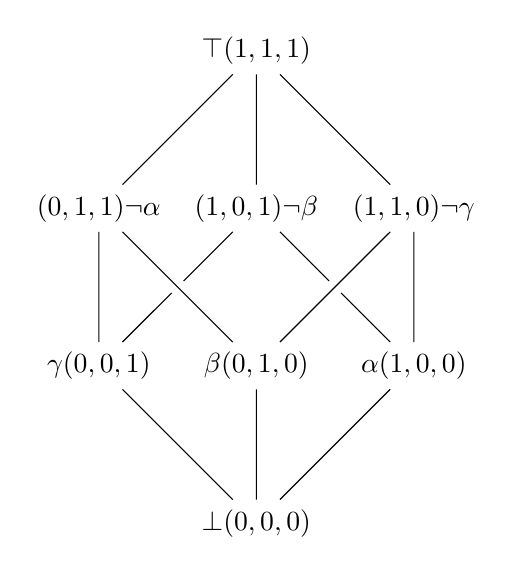
\begin{tikzpicture}
  \node (max) at (0,4) {$\top (1,1,1)$};
  \node (a) at (-2,2) {$(0,1,1)\neg\alpha$};
  \node (b) at (0,2) {$(1,0,1)\neg\beta$};
  \node (c) at (2,2) {$(1,1,0)\neg\gamma$};
  \node (d) at (-2,0) {$\gamma(0,0,1)$};
  \node (e) at (0,0) {$\beta(0,1,0)$};
  \node (f) at (2,0) {$\alpha(1,0,0)$};
  \node (min) at (0,-2) {$\bot (0,0,0)$};
  \draw (min) -- (d) -- (a) -- (max) -- (b) -- (f)
  (e) -- (min) -- (f) -- (c) -- (max)
  (d) -- (b);
  \draw[preaction={draw=white, -,line width=6pt}] (a) -- (e) -- (c);
\end{tikzpicture}
  \label{fig:boolean_algebra}%
\end{marginfigure}

\noindent First observe that 

\begin{equation}
\begin{split}
[ \alpha \text{ if } Neutral, \omega \text{ if } \neg Neutral ]_{contract_{1}} \\  \sim [ \omega  \text{ if } Neutral, \alpha \text{ if } \neg Neutral ]_{contract_{2}} \\   \Rightarrow u(contract_{1})  = u(contract_{2})   \\  \Rightarrow EU(contract_{1}) \\ = u(\alpha)p(Neutral) + u(\omega)(1-p(Neutral)) \\ 
= u(\omega)p(Neutral) + u(\alpha)(1-p(Neutral)) \\ 
= EU(contract_{2})  
\\ \Leftrightarrow p(Neutral) = 0.5
\end{split}
\end{equation}

\noindent Then we can take any two extremes $u(\alpha) = 1, u(\omega) = 0$ and we can use our test for indifference to situate any third proposition $\gamma$ on a desirability scale since: 
\begin{equation} 
\begin{split}
 [\gamma \text{ if } Neutral, \gamma \text{ if } \neg Neutral]_{contract_1} \\ 
 \sim   [\alpha \text{ if } Neutral, \omega \text{ if } \neg Neutral ]_{contract_2} \\
 \Leftrightarrow EU(contract_{2}) = u(alpha)\frac{1}{2}  + u(omega)\frac{1}{2} = .5  \\ = u(\gamma) = EU(contract_{1})
\end{split}
\end{equation}

Repeating this step we can find a contract on a sure-thing $\psi$ for which we're indifferent between:
\begin{equation} 
\begin{split}
[\psi \text{ if } Neutral, \psi \text{ if } \neg Neutral]_{contract_1}  \\
 \sim   [\alpha \text{ if } Neutral, \gamma \text{ if } \neg Neutral ]_{contract_2} \\
  \Rightarrow u(\psi) = .75
   \\ . . . etc
 \end{split}
\end{equation}

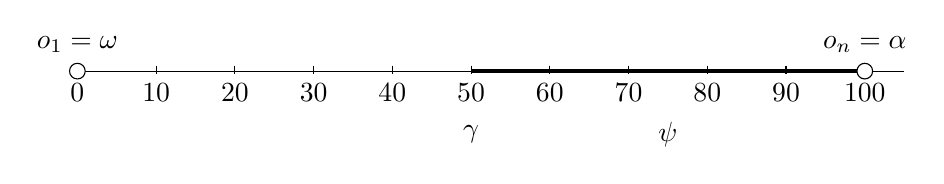
\begin{tikzpicture}
% a straight line segment
\draw (0.1,0) -- (10.5,0);
% the ticks and their labels
\foreach \x  in {0,...,10}
  \draw[xshift=\x cm] (0pt,2pt) -- (0pt,-1pt) node[below,fill=white] {\the\numexpr\x*10\relax};
% the thicker segment
\draw[ultra thick] (5,0) -- (10,0);
% the labels
\node[fill=white,draw=black,circle,inner sep=2pt,label=above:{$o_1=\omega$}] at (0,0) {};
\node[fill=white,draw=black,circle,inner sep=2pt,label=above:{$o_n=\alpha$}] at (10,0) {};
\node at (5,-0.8) {$\gamma$};
\node at (7.5,-0.8) {$\psi$};
\end{tikzpicture}

Repeating this process indefinitely we can refine our utility scale as exactly as we please, by repeatedly finding prospects with a utility precisely  on the mid-point between two poles. If these measures adhere to certain basic constraints of rationality regarding consistency of utility we can show how a Bayesian agent can be seen to maximise their expected utility when making decisions under uncertainty. But unlike the Von Neumann representation theorem, for a Bayesian the probability function over prospects is not unique. We can have multiple pairs $\langle p, u \rangle$ which are representative of an individual's preference ordering $\succeq$ without converging on the particular probabilities ascribed by one individual. This is precisely the content of the following theorem. 

\begin{ftheo}{Bolker Representation Theorem}
\label{section:BolkersRepresentation}
Let $ \mathbb{B} =  \langle \Omega, \succeq \rangle $ be Bolker structure if $\Omega$ is an atomless Boolean algebra and $\models$ forms an implication relation over $\Omega$, while $\succeq$ is complete, transitive, continuous over $\Omega \setminus \bot$ and the following hold: 
\begin{enumerate}
\item (Impartiality) Suppose $\alpha \sim \beta $ and $\exists \gamma (\neg(\gamma \sim \alpha))$ such that  $\alpha \wedge \gamma = \bot = \beta \wedge \gamma$ and $\alpha \vee \gamma \sim \beta \vee \gamma $ Then $ \forall \gamma ( \alpha \vee \gamma \sim \beta \vee \gamma )$ 
\item (Averaging) If $\alpha \wedge \beta = \bot$ then $\alpha \succeq \beta \Leftrightarrow \alpha \succeq \alpha \vee \beta \succeq \beta$
\end{enumerate}
Then there is a probability measure and utility (desirability) metric $\langle p, u \rangle$ on $\Omega$ such that if the following axioms hold:
\begin{itemize}
\item (A0) $p(\top) = 1$
\item (A1) $p(\alpha) \geq 0$
\item (A2) $\alpha \wedge \beta = \bot \rightarrow p(\alpha \vee \beta) = p(\alpha) + p(\beta)$
\item (A3) $u(\top) = 0$
\item (A4) ${\alpha \wedge \beta = \bot \wedge p(\alpha \vee \beta) \neq 0}$  implies  ${u(\alpha \vee \beta) = \dfrac{u(\alpha)p(\alpha) + u(\beta)p(\beta)}{p(\alpha \vee \beta)} }$
\end{itemize}
it follows that
$$  u(\alpha) \geq u(\beta) \Leftrightarrow \alpha \succeq \beta $$

and there is another such set of functions $\langle p^{*}, u^{*}    \rangle$ if and only if $u^{*}$ is a fractional linear transformation of $u$ i.e. ${ \exists a > 0}$ and ${\exists c , cu(\alpha) > -1}$
$$ p^{*}(\alpha) = p(\alpha) \cdot (cu(\alpha) + 1) $$
$$u^{*}(\alpha) = \frac{au(\alpha)}{cu(\alpha)+1} $$
\end{ftheo}

The mathematical machinery used to prove this result is a little more involved, ranging over every possible boolean combination of beliefs measured on three axes: preference, probability and desirability. In addition to the usual probability axioms, (A3) and (A4) tie subjective probability and subjective utility together. The axiom (A3) works to normalise the utility scale so that no sure prospect has any positive utility. This, in a sense, enshrines the requirement that there is only a utility to novel information. While (A4) ensures that the utility of any disjunction is the weighted average of the ways in which it can occur. More importantly it implies:
 $$u(\alpha \vee \neg\alpha) = u(\top) = p(\alpha)u(\alpha) + p(\neg\alpha)u(\neg\alpha)$$  
 $$= p(\alpha)u(\alpha) + u(\neg\alpha) - p(\alpha)u(\neg\alpha) $$
 $$ \Rightarrow u(\top) - u(\neg\alpha) = p(\alpha)u(\alpha)  - p(\alpha)u(\neg\alpha)$$
 $$ \Rightarrow p(\alpha) = \frac{u(\top) - u(\neg\alpha)}{ u(\alpha)  - u(\neg\alpha)} \text{  if } u(\alpha) \neq u(\neg\alpha) $$ 
Which confirms how the relationship between probability of a given proposition can be expressed in terms of the desirability or utility of the same proposition and it's negation. This is a view of probability profoundly different from measure of risk we ascribe to players calculating pot-odds in poker. It is not a fixed unique distribution determined by observation across repeated sampling, and consequently much harder to model. The probabilities reflect the dynamics and eccentricities of individual beliefs and the agent is seen as maximising their subjective expectations. Given how the average consumer cannot then be modelled with respect to a fixed reference probability distribution, you might despair of ever predicting an individual's actions. Fortunately crowding promotes conformity and what seems mysterious at the micro level becomes clearer at the macro scale.

\section{\textbf{Part IV: Machine Learning and the Customer}}

\subsection{Customer Representation: A Segmentation Approach}
\label{sec:Segmentation}
Having arrayed all the ingredients of a consumer utility model and the traditional theorems used to motivate the idea, a few things might cross your mind: (1) This notion of subjective utility would be useful, but seems incredibly hard to pin-down. (2) how for any given individual can we reasonably ascribe either a motivating utility curve or probability measure? (3) Even if we could elicit their preferences, there is no guarantee that the preferences are stable or entirely consistent. (4) Nor is it clear how we could (at any kind of scale) garner those expressed preferences. (5) Surmounting all these obstacles, we still have no way to assume they're going to pursue their maximum expected value as opposed to adopting an alternative decision rule! In other words, this theory is about how we should act, not how we do act. The practical constraints of sampling preferences at sufficient scale make the attribution of individual utility profiles impractical. This is all true as far as it goes, but the influence of the above theorems and the utility model of rational choice lies in the perspective it offers, not the recipe it prescribes.
\linebreak

\noindent Although there have been some brave attempts to derive customer utility metrics from survey data \footnote{Discussed in \cite{HalpernReasoning}pg 187}, the typical approach to modelling customers ignores the subtleties of directly estimating a utility function in favour of a look-alike predictive approach; customer segmentation and product recommendations based on the actions of similar customers in the past. It's easier to model customers in the aggregate than in the particulars. Easier again to model our own preference than placate the consumer. 

\subsection{PCA and Segmentation}
Treating the customer as commodity with a limited range of behaviour puts us back in the business of sampling. We treat each interaction as instance of behaviour fluctuating around a predictable pattern. This is comforting because it's familiar and seemingly absolves us about attributions of utility and the burden of interpretation. This is illusory. While there is a wide range of segmentation methods which can be applied to the task of classifying both customers and products. These classification schemas are vital inputs for any recommendation algorithm. They cluster individuals based on a wide array of features, which is to say that they simplify the question of expected action. Instead of asking how might Rebecca, (aged between 18-25, from Spain, with a history of frugal purchases) react to a new sales promotion, you can ask about the conversion rate of the young female demographic. Depending on the task and the nature of the clustering algorithm, you might end up bucketing Rebecca with Sven (overweight male, history of lavish spending from Sweden) if, for example, their historic email open rates were similar. The responsibility for vetting each clustering schema lies with the user of the algorithm, but usually knowledge of the problem is enough to put some kind of context on the structural patterns unearthed by the algorithm. 
\linebreak

\begin{table}[htb]
\centering
\sffamily
\caption*{Customer Features}
\begin{tabular}{l*{4}{c}}
\toprule
 \bfseries Customer ID & \bfseries custDesc0 & \bfseries custDesc1 & \bfseries ... & \bfseries CustDescN \\
\midrule
\texttt{1}      & 3.2               & 4.5                 & ...                 & 10               \\
\texttt{2}   & 5.2               & 4.3                 & ...                  & 8.2              \\
\texttt{3} & 5.6              & 4.2                 & ....                & 8.5              \\
\texttt{4}     & 7.5              & 4.6                 & ...                 & 12               \\ \bottomrule
\end{tabular}
\end{table}

\noindent Ideally we would parse out our data into the most relevant descriptive features, but in lieu of domain knowledge we can apply some data compression techniques such as principle components analysis to extract latent features in the data. These techniques are dangerous when applied without domain knowledge or some kind of supervision. A technique, in the same vein as PCA, called factor analysis tries to construct latent factors from correlations in the observed features. Historically this was abused to measure "intelligence" as a latent factor driving performance on aptitude tests. So while we should be wary of over-inflating artefacts of the data, the technique is useful for finding structure. Starting from the covariance matrix of the scaled customer data :

$$ Cov(\mathbf{X}) = \operatorname{cov}[X_i, X_j] = \operatorname{E}[(X_i - \operatorname{E}[X_i])(X_j - \operatorname{E}[X_j])]
$$

\begin{marginfigure}
\includegraphics[width=3in, height=5.in]{Plots/pca_explained_variance.png}
\caption{Principle Component Analysis of Customer Features}
\end{marginfigure}

\begin{minted}{python}
X = df_customer[[x for x in df_purchases.columns 
if 'customer_desc' in x]]
X_std = StandardScaler().fit_transform(X)
## Covariance Decomposition
cov_mat = np.cov(X_std.T)
eig_vals, eig_vecs = np.linalg.eig(cov_mat)
## Explained Variance
tot = sum(eig_vals)
var_exp = [(i / tot)*100 for i in sorted(eig_vals, reverse=True)]
cum_var_exp = np.cumsum(var_exp)
\end{minted}

\noindent For any observed set of customer attributes, their covariance matrix can be factorized (or decomposed) into a matrix product of the eigenvectors and eigenvalues. These components can in turn be analysed to express the manner in which each of the original features contributes to the new construct. Each component captures a proportion of the total variance observed in the original covariance matrix:

\begin{marginfigure}
\includegraphics[width=3in, height=5.in]{Plots/pca_component_weights.png}
\caption{Principle Component Weightings by Observed Customer Features}
\end{marginfigure}

\noindent If we're lucky, a small number of the eigenvectors (principle components) can be shown to explain the variance in the data (as in Figure 17) and thereby represent a complex customer problem in a reduced dimensional space. Each customer is visualised as a complex of observed characteristics along the axes of the principle components in, for example, a two dimensional plane. Furthermore, we can overlay an interpretation on the components by associating group identifiers to portions of the plane. In the dataset pictured in Figure 19 we've tried to represent the data in three groups inferred by a k-means clustering algorithm over the original observed features. This is not the most appropriate categorisation as can be seen by the manner in which 9 clear cohorts are speckled across the space. In other words there is more diversity in our customer base than the clustering is capable of expressing. That's not to say all diversity needs to be captured. If our purpose is make the broadly correct action (e.g. sell, promote, no-action), the niceties can often be ignored. A Silhouette score analysis shows that one of our classes is too crude, collecting dissimilar customers together. Nevertheless, the expected value of the customer is then something like the probability of purchase (however approximated) for the given customer multiplied the the net revenue of the average purchase in the same group. It's these kind of idealisations and conceptual economies, which seemingly reasonable at the time, lead to systematic algorithmic skew. Unrefined constructs encourage brutish bulk actions across the arrayed field of customers. 
\linebreak

\begin{marginfigure}
\includegraphics[width=3in, height=5.in]{Plots/pca_representing_clusters.png}
\caption{Principle Component Representation of Customer Clusters}
\end{marginfigure}

$$ EU^{seg}  = \sum_{i=1}^{i=n} p^{seg_{i}}u^{seg_i} $$


\noindent Note the level of abstraction here! In an effort to understand the customer as a predictable entity we've gone from a set of concrete but complex customer descriptions through a matrix decomposition representation of their variant behaviours, then focused on a weighted sum construct of the observed behaviours that in some sense best "explain" the diversity of the behaviours in the original data. Concluding with a group-categorisation of how that behavioural construct can be interpreted or acted upon. The grouping is key. If the complexities of the model is a wound demanding attention. The segmentation is the interpretable overlay which is sold to your management, it's the salving balm of targeted advertisement sold to investors.

\begin{marginfigure}
\includegraphics[width=3in, height=5.in]{Plots/silhouette_scores.png}
\caption{Cluster Validation by Silhouette scores - a customer measure of similarity within and across the available clusters.}
\end{marginfigure}

\noindent So in practice there is some constraints of "plausibility" applied to these kinds of models. But once the model is live in productions it becomes hard to correct for anything other than degrading performance on the metric that matters most; expected value. 

\section{\textbf{Conclusion: Construct Criticism}}
The theory of expected value has been around for a long time. It has been criticised and corrected, adjusted  and refined. We've seen two broad species of justification for the rule: (1) a random process will converge around a stable mean in the long-run by the law of large numbers, so better to maximise that mean, (2) the procedure is justified by appeal to the representation theorem and the various axiom schemes of rationality. In practice, both encounter difficulties as described above. We can rarely justify the time or resources required for long run convergence since most questions are more urgent, and there are regular examples of humans violating the principle when faced with a decision. A number of apparent paradoxes where following the paradigm would result in reputedly irrational results. Moves and counter-moves in the debate. Straw-men are built and burnt, but the back and forth is beyond the scope of this blog post.\footnote{A good discussion can be found in\cite{BinmoreRational}} Nevertheless even with radically different approaches to modelling customer preference, concerns about expected value will permeate all proposed solutions. It is a metric, explanation and a soothing, bloodless formula. 
\linebreak

\noindent Yet the model constructs which feed the formula are not neutral; on the one hand you may question the sample data, on the other there are fair questions about the design choices that go into constructing the models. Did your data capture the correct features? Were you able to extract the important structural regularities? Did we run the experiment for long enough? Was the sample biased? Is the attributed probability still valid, are the utility curves steep enough? Does the clustering scheme make sense? When the model design is filtered through the expected value metric, the subtleties of those choices get glossed over and obscured. The creative leaps and structural assumptions calcify, become heuristics and accrue advocates and devotees. Analysts masquerade as oracles claiming as wisdom formulas carved in clay on crumbling architecture. The irony here is sharp. In both the Von Neumann and Jeffrey's formulation, decision theory is an inescapably constructive project - directly responsive to the polled preferences of dynamic individuals across a variety of different domains, subject to differing axioms as appropriate. Yet, stasis is the inevitable result from cleaving too tightly to a simple metric like expected value. Improvements are made and measured in minor swings around the sink-hole of local optima, if you're lucky. More likely, in a market context, the simple minded pursuit of a single KPI leaves you vulnerable to exploitation. Without regular attention these model constructs lose relevance and compound the errors of the past. The simple rule is often too simple. 


\bibliography{library}
\bibliographystyle{plainnat}

\end{document}



